\documentclass[conference]{IEEEtran}
\IEEEoverridecommandlockouts
\usepackage{cite}
\usepackage{amsmath,amssymb,amsfonts}
\usepackage{algorithmic}
\usepackage{textcomp}
\usepackage{graphicx}
\usepackage{lipsum}
\usepackage{tabularx}
\usepackage{booktabs}
\usepackage{multicol}
\usepackage{xcolor}
\usepackage{amsmath}
\usepackage[numbers]{natbib}
\usepackage{adjustbox}
\graphicspath{ {images/} }

\begin{document}

\title
{
    Energy Efficient Path Planning on A Legged Robot\\
    \author{Robbie Buck, Joseph Ditton, Carter Bailey, Max Thomas}
    \thanks{All authors are affiliated with the Department of Computer Science, Utah State University, Logan, UT, 84321 USA}
}
\maketitle

\begin{abstract}
    Sampling Based Model Predictive Optimizer (SBMPO) is an energy efficient path planner designed for kinodynamic robots. SBMPO is supposed to always find the most energy efficient path to its goal, but this has only ever been proven in simulation. This paper presents the results from testing SBMPO on a real robot and seeing if it is still able to find the most energy efficient path.
\end{abstract}

\begin{IEEEkeywords}
\\ Energy Efficient Path Planner, Legged Robots
\end{IEEEkeywords}

\section{Introduction}
    
    % intro para - Talk about benefits of legged robots over other types
    \IEEEPARstart{L}{egged} robots are becoming more popular to use due to their ability to traverse terrain that wheeled robots cannot. Legged robots consume energy more quickly than their wheeled counterparts due to more motors being involved to keep the robot standing and moving. This increase in energy consumption makes it so that energy efficient path planning for legged robots is critical. 
    
    \begin{figure}[ht]
        \centering
        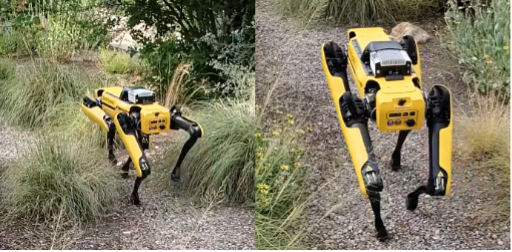
\includegraphics[width=0.47\textwidth]{spot_walking}
        \caption{Legged Systems have the ability to traverse terrain that wheeled systems cannot but have a limited power supply.}
        \label{fig:spot_walking}
    \end{figure}
    
    % talk about energy efficient path plan needs for legged robots
    The research presented in this paper tests and compares an energy efficient path planner to other common path planners (A-Star, Dijkstras). Energy efficient path planners usually have to explore more to find the most energy efficient path. This results in a longer convergence time and slower updates to path planning when a robot is planning a route while on the move. By comparing energy consumptions of these path planners, it can be seen if an energy efficient path planners extra convergence time is worthwhile for a legged robot when traversing terrain. 
    
    % close out with summary of what our research is doing
    Our research has shown that our tested energy efficient path planner is able to find better energy efficient paths the majority of the time. These results cause us to believe that as energy efficient path planner convergence times are lowered they will be used more in the real world to extend the work time of robots. 
    
\section{Literature Review}

    Modern robots come in many shapes and sizes. Typically, robots are either wheel-based, manipulators, or model "animal-like" behavior \cite{BING2020323, 8946895, mario}. Wheeled robots are common because their kinematics are simpler, and they can carry large payloads. Manipulators have been around the longest, but their applications are limited. "Animal" robots, specifically legged robot systems, are gaining momentum because of their versatility, including the ability to move on and through unstructured terrain.
    
    Legged robots are beneficial because they can traverse terrain not available to wheel-based robots. However, the kinematics are far more complicated and the payload capacity is significantly lower. Due to these constraints, energy is a premium. Thus, energy efficient path planners are important for legged robot research \cite{mario, aau5872}.
    
    Intuitively, minimizing the distance travelled will aid in lowering energy consumption. This works well in simple, consistent environments, but in nature where the environments are variable and complex, many animals plan according to a conceptual measurement of how much energy will be expended on a given path \cite{mousas2013minimum}. This same strategy applies to robots. Planning to avoid difficult terrain or maximizing the amount of time spent in the sun to facilitate photo-voltaic power generation can reduce the amount of net energy expenditure at the cost of taking a longer path \cite{plonski2013energy, wu2019energy}.
    
    Determining an energy cost for different types of terrain is a strategy that can be integrated into nearly every path-planning algorithm \cite{mousas2013minimum}. Knowing beforehand the cost of each expected class of terrain can reduce complexity during the planning phase of robot locomotion, though some attempts have been made to determine cost in real-time with some success \cite{howard2007optimal, plonski2013energy, iagnemma2004online}.
    
    The Boston Dynamics SPOT robot is the platform used during the research presented in this paper. SPOT's standard battery provides around 60 minutes of power under normal conditions. Additional hardware, such as an external battery module, and high efficiency voltage regulators can improve SPOT's efficiency or enable the use of additional sensors that require more energy \cite{bouman2020autonomous}.
    
    It is important for robots to be able to identify their actual position when path planning. The most common tactic for estimation is dead reckoning, where the robot estimates its position based on motor movement or other internal measurements, without the aid of outside sensors \cite{komoriya1994position}. Camera, lidar, sonar, gyroscopes, and GPS can all be used to improve location estimation \cite{8460940, drumheller1987mobile, westmore1991direct, komoriya1994position}.
    
    As will be discussed later in this paper, SPOT uses its cameras for estimating velocity, which in turn can be used to estimate location. We found this estimate to be unreliable in some circumstances, so investigating other methods of estimation was pertinent. For position estimation, GPS is an appealing choice. Additionally, given a high level of accuracy and frequent enough updates, GPS data can be used to extrapolate kinematic state, namely the velocity of the robot \cite{witte2005accuracy}. GPS might not be accurate enough in poor weather or indoors to be sufficient for path planning so consideration should be taken given those limitations \cite{8460940}.
    
    Energy efficiency is tightly correlated with both linear and angular velocity and this relationship has been well explored for wheeled robots \cite{mei2004energy, barili1995energy}. For legged robots, gait also has an effect on energy consumption and lower-level directives, like balance, generally have higher priority \cite{roy2012effects}. While this paper doesn't discuss SPOT's gait, we recognize that this will have an affect on energy consumption, particularly when SPOT is executing a turn.


\section{Methods}
    \subsection{SBMPO}
        Legged robots have an advantage over wheeled robots when it comes to the type of terrains they can traverse, but this versatility comes at the cost of energy efficiency \cite{leggedRobots, silva2012literature, aau5872, mario}. Due to the reduced carrying capacity, legged robots cannot carry as big of batteries as their wheeled counterparts; thus, energy efficiency for legged robots is a premium. The SPOT robot's battery provides power for around 60 minutes of normal operation - limiting the types of activities and responsibilities that SPOT can perform to shorter tasks.
        
       \begin{figure}[h]
           \centering
           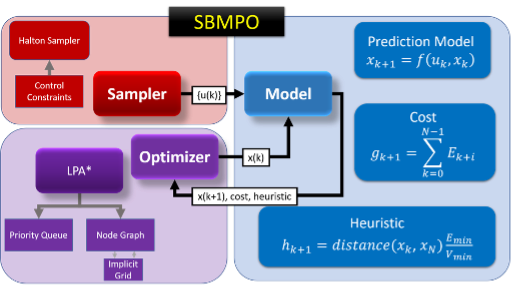
\includegraphics[width=0.47\textwidth]{SBMPO}
            \caption{SBMPO core components. SBMPO is comprised of three major components: A sampler that determines what control input is explored, model-specific functions, and an optimizer based on a A*-type algorithm.}
            \label{fig:SBMPO}
        \end{figure} 
        
        % 2nd Paragraph talk about how energy efficient path planners have been designed and then focus in on SBMPO
        In order to maximize the battery life of SPOT, we propose to test an energy efficient path planner, Sampling Based Model Predictive Optimization (SBMPO) \cite{mario}, and compare the energy costs of SBMPO to two other commonly used path planners A-Star and Dijkstras \cite{duchovn2014path, wang2011application}. We choose to employ SBMPO for its ease of use with legged and dexterous mobility robots, and its demonstrated energy efficient path planning capabilities on both legged and wheeled ground robots \cite{mario}.  
        
        % 3rd paragraph hone in on SBMPO and politely copy (steal 笑う) the paragraph Mario wrote about SBMPO from my last paper
        SBMPO works with a variety of dynamic holonomic or non-holonomic robot models, either linear or nonlinear. These models may be derived from first principles or learned, and can also be non-invertible as SBMPO samples the input (i.e., control) space directly, alleviating the cumbersome need for local connection planners or inverse kinematics. 

    \subsection{Collecting Data from Spot}
        To allow SBMPO to calculate energy efficient paths for SPOT, SBMPO needs to know the energy consumption that occurs when spot is making specific angled turns at 1 m/s. This research aimed to test SBMPO on three separate terrains to see how accurate SBMPO was in different environments. The terrains that data was collected on was grass, gravel, and concrete. 
        
        \subsubsection{SPOT's Built in Speed Sensor}
            Initial attempts at collecting the turning energy cost data from SPOT proved fruitless because even though SPOT was given commands to go a certain speed at a certain angle. SPOT's estimated speed would vary dramatically as it made the turn. This speed inaccuracy was due to SPOT using its built in cameras to estimate its speed. The initial data that was collected during this run is shown in \ref{fig:cameraPowerCost}. 
            
            \begin{figure}[ht]
                \centering
                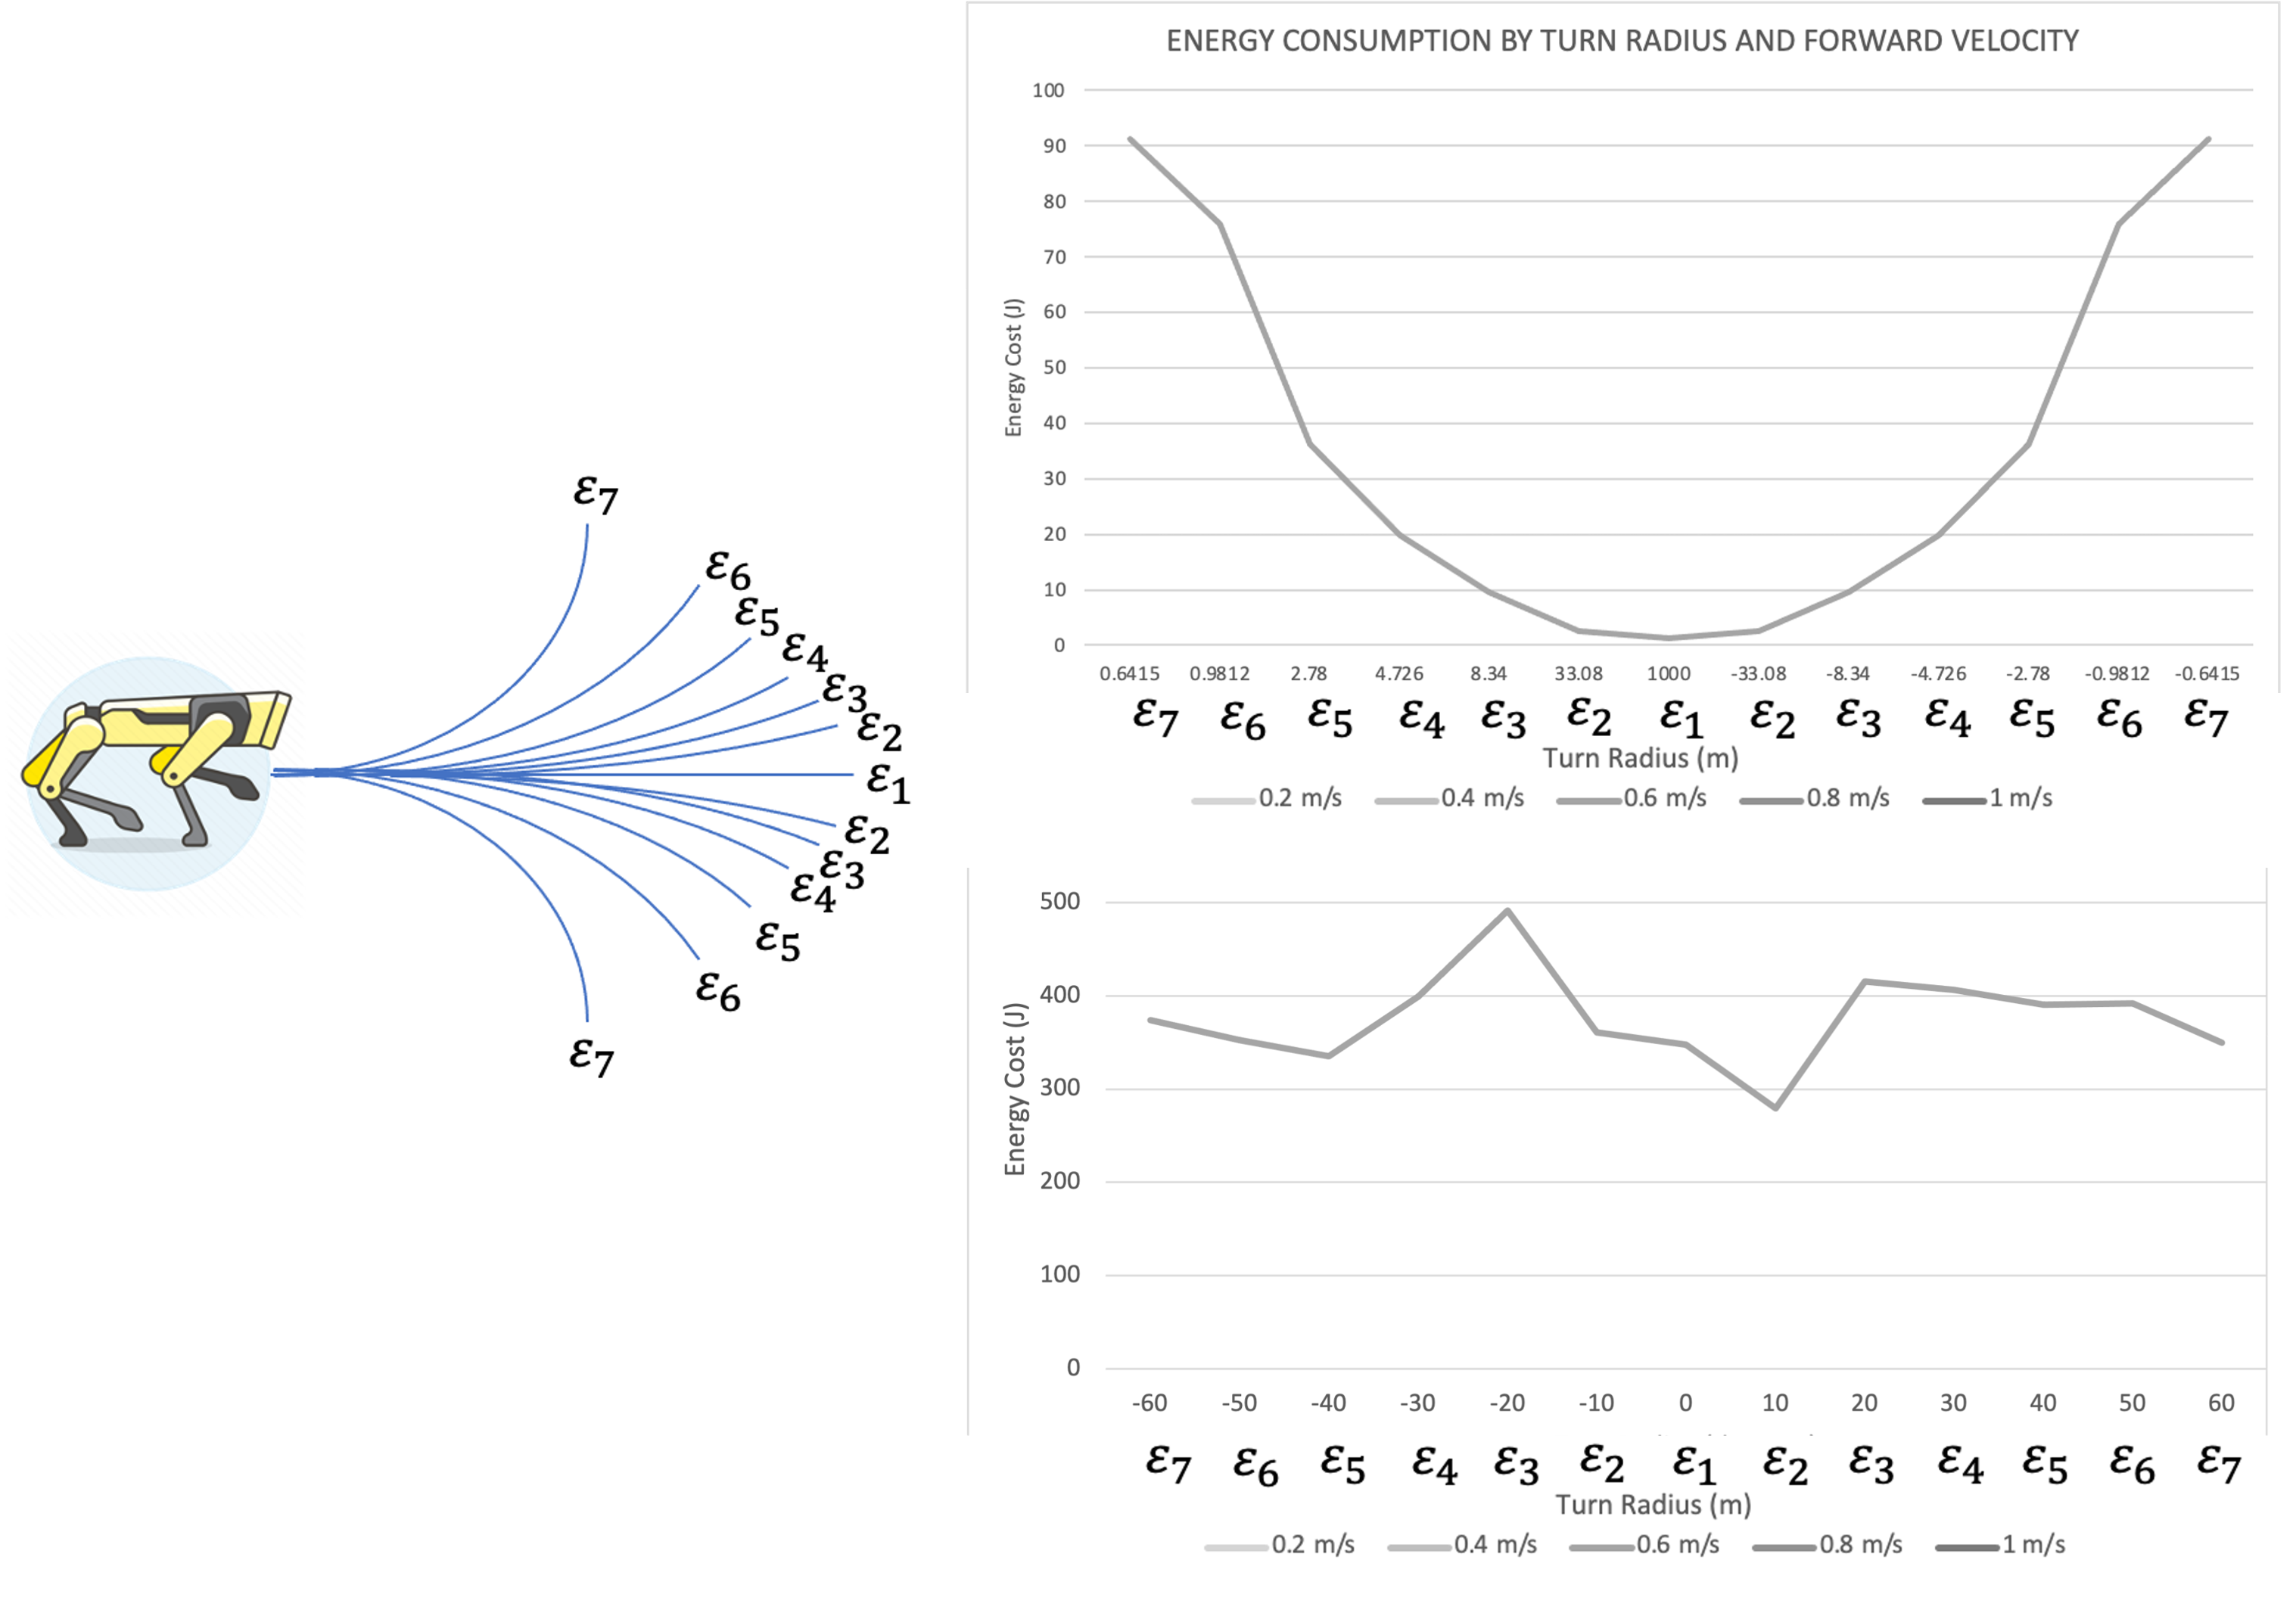
\includegraphics[width=\linewidth]{turnRadius.png}
                \caption{An expected power output as SPOT moves is shown on the upper graph while the initial power outputs that were collected when SPOT was using its cameras for speed detection is shown on the lower graph.}
                \label{fig:cameraPowerCost}
            \end{figure}
            
            To increase SPOT's speed estimate accuracy, Boston Dynamic's provides tags that can be put in the environment that SPOT is being used in. These tags did increase SPOT's accuracy on speed estimates when walking towards a tag directly. But once SPOT started to turn, the benefits of using the tag were lost. Since accurate speed readings when turning were needed the team decided to use a GPS system.\\
            
        \subsubsection{GPS}
            The GPS system that was used for speed data collection was an EMLID Reach. The EMLID Reach system uses a base station that is static which then communicates with smaller GPSs. Two smaller GPS systems were attached to SPOT and then connected to the base station. The data that was obtained using this method was centimeter level accurate. Using this method, we were able to collect the energy costs of specific angled turns with high accuracy on three terrains.
            
            The EMLID system allowed accurate speed estimates with timestamps that could be matched up to SPOT's power output. This allowed for the creation of the turn angle costs that SBMPO required to accurately provide energy efficient paths for SPOT.
            
\subsection{Testing SBMPO on SPOT}
    
    % Talk about the obstacle fields and how they were designed
    Once the energy costs for specific turns were provided to SBMPO for SPOT, initial testing could occur. The obstacle fields for all terrains were man-made so that they could be easily replicated on all terrains that were being tested on. The majority of the man-made obstacle fields were designed to cause the robot to take a different path depending on if SBMPO, A-Star, or Dijkstras was run on SPOT. This allowed us to easily compare power output differences for the two path planners. An example path is shown in Figure \ref{fig:spotWithObstacles}.
    
    % Talk about how we compared the results of SBMPO to another path planner. A-Star?
    On the obstacle fields that SBMPO, A-star, and Dijkstra produce similar routes on, the power output difference will be smaller. The power differences are mainly visible during turns where A-Star and Dijkstra will focus on taking the quickest turn whereas SBMPO will take the most energy efficient.
     
    \begin{figure}[ht]
    \centering
    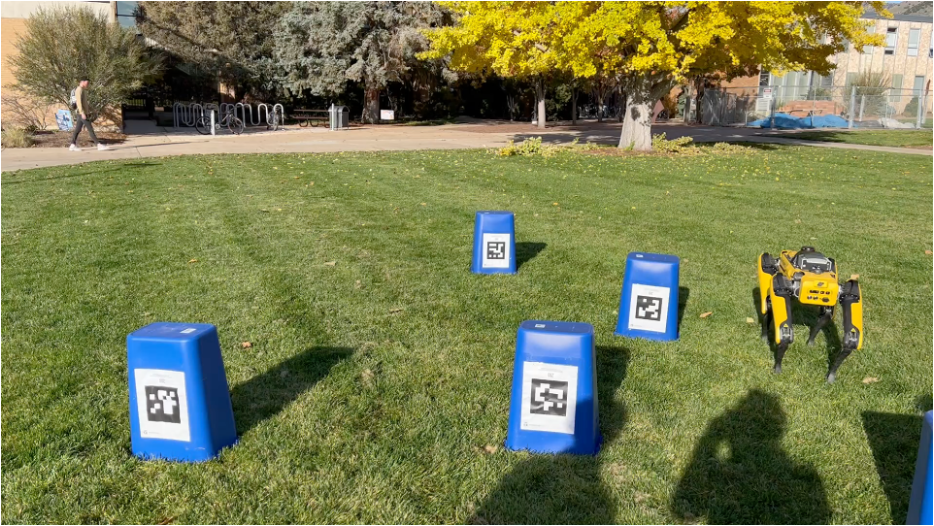
\includegraphics[width=\linewidth]{obstacles.png}
    \caption{An example of a course that SBMPO was expected to provide an energy efficient path for SPOT to traverse through. The goal location is in the lower left corner of the image.}
    \label{fig:spotWithObstacles}
    \end{figure}
     
\section{Results}
    \subsection{Power Consumption}
    \subsubsection{Turn Angles}
    Traditional robots such as wheeled robots typically have a predictable power consumption profile. As the turn angle increases, power increases. However, initial results with SPOT show a different picture. Figures 5 and 6 show power consumption for various turn angles for SPOT. In this particular path, the 40 degree right turn angle was the most costly, and both 10 degree turns were less costly than walking straight. Also noteworthy, 60 degree turn angles were both far less costly than 50 degree turns.  
    
    \begin{adjustbox}{center, caption={Power Consumption for various turn angles},nofloat=figure}
        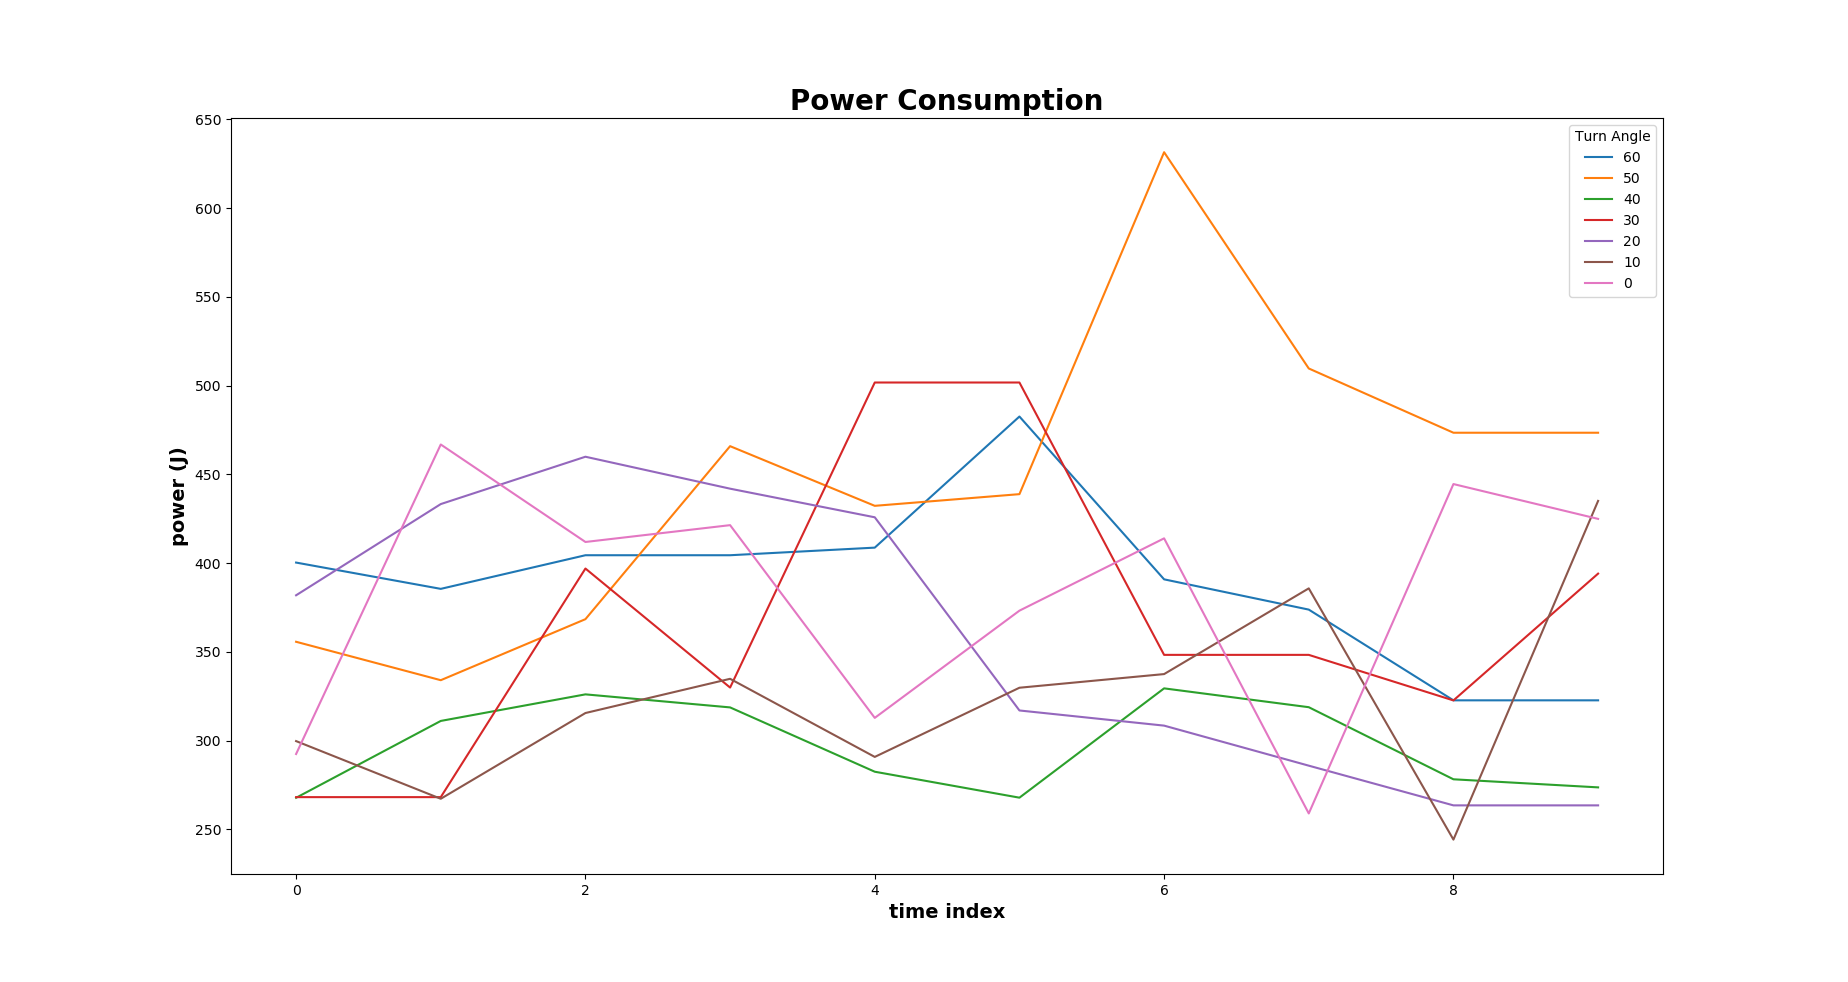
\includegraphics[width=1\linewidth]{power_turnRadius.png}
    \end{adjustbox}
    
    \begin{adjustbox}{center, caption={Average Power Consumption per turn angle}, nofloat=figure}
        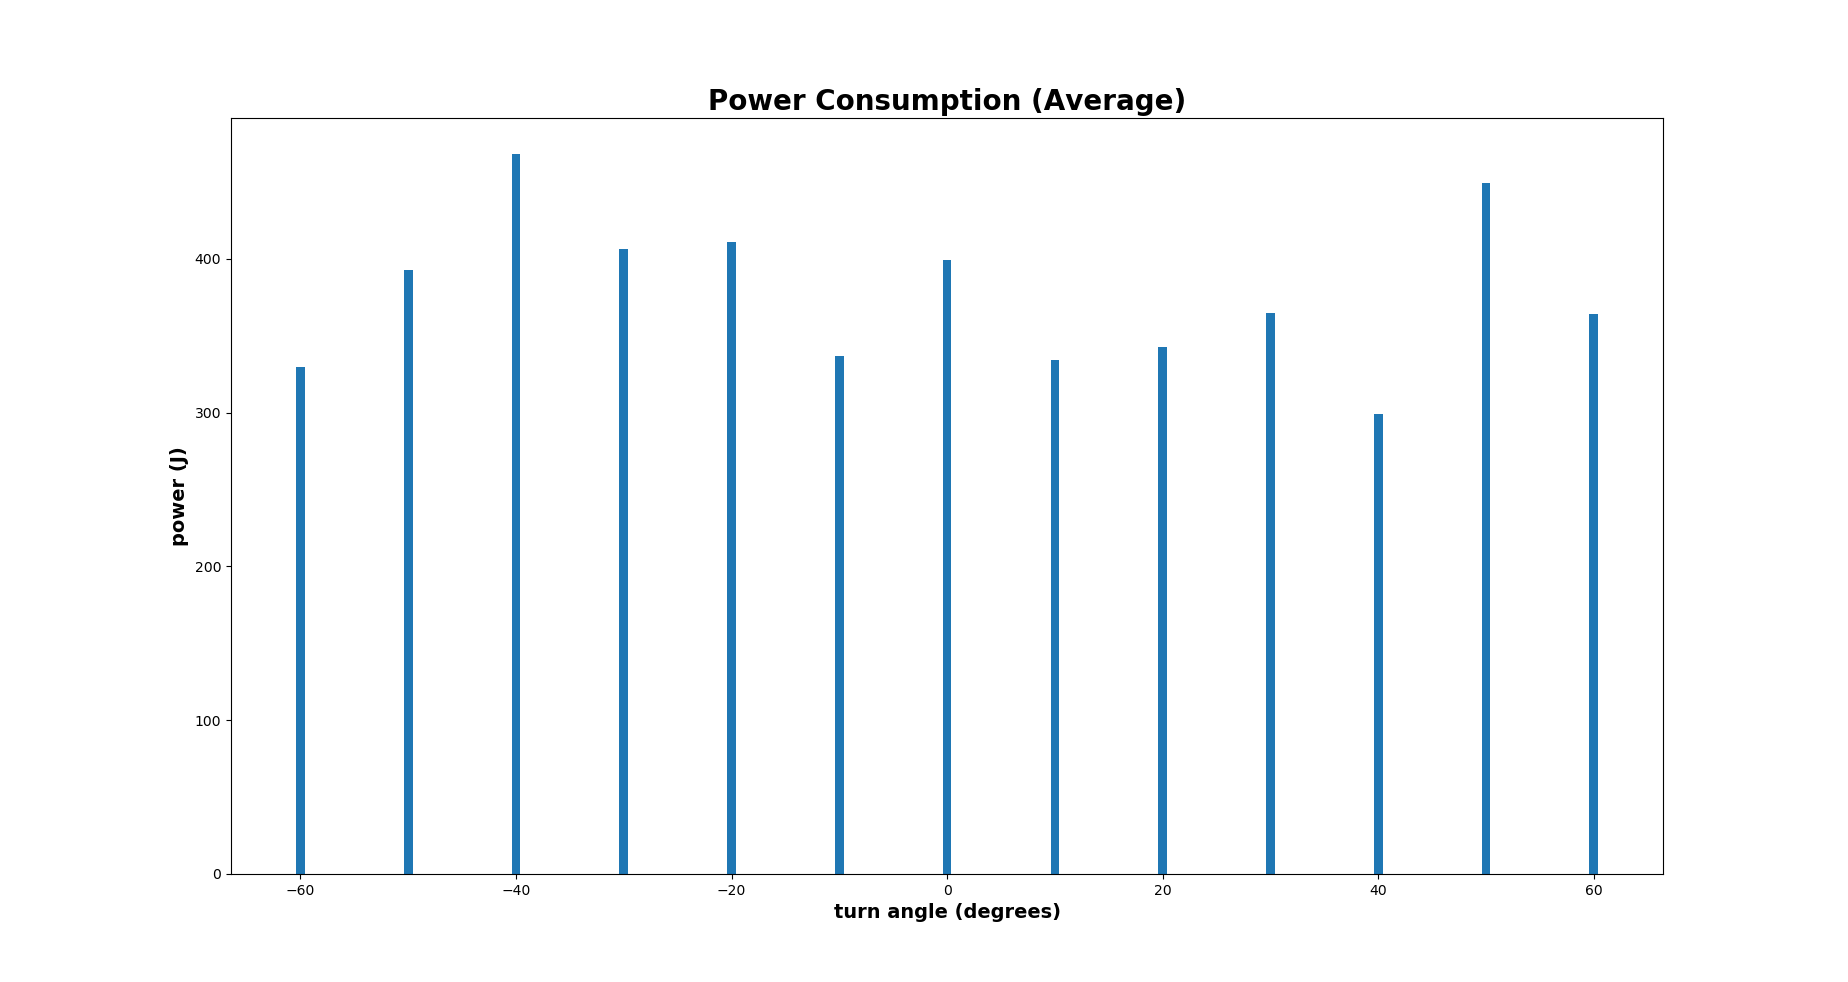
\includegraphics[width=1\linewidth]{power_avg.png}
    \end{adjustbox}
    
    \subsubsection{Terrains}
    Figure 7 shows a comparison of power consumption over various turn angles for multiple terrains. Specifically, we collected data for SPOT on grass, asphalt, and gravel. Asphalt appears to require the most energy, whereas grass consumes the least power overall. All terrains fail to show a predictable power consumption pattern for turn angles.
    
    \begin{adjustbox}{center, caption={Power Consumption terrain comparison}, nofloat=figure}
        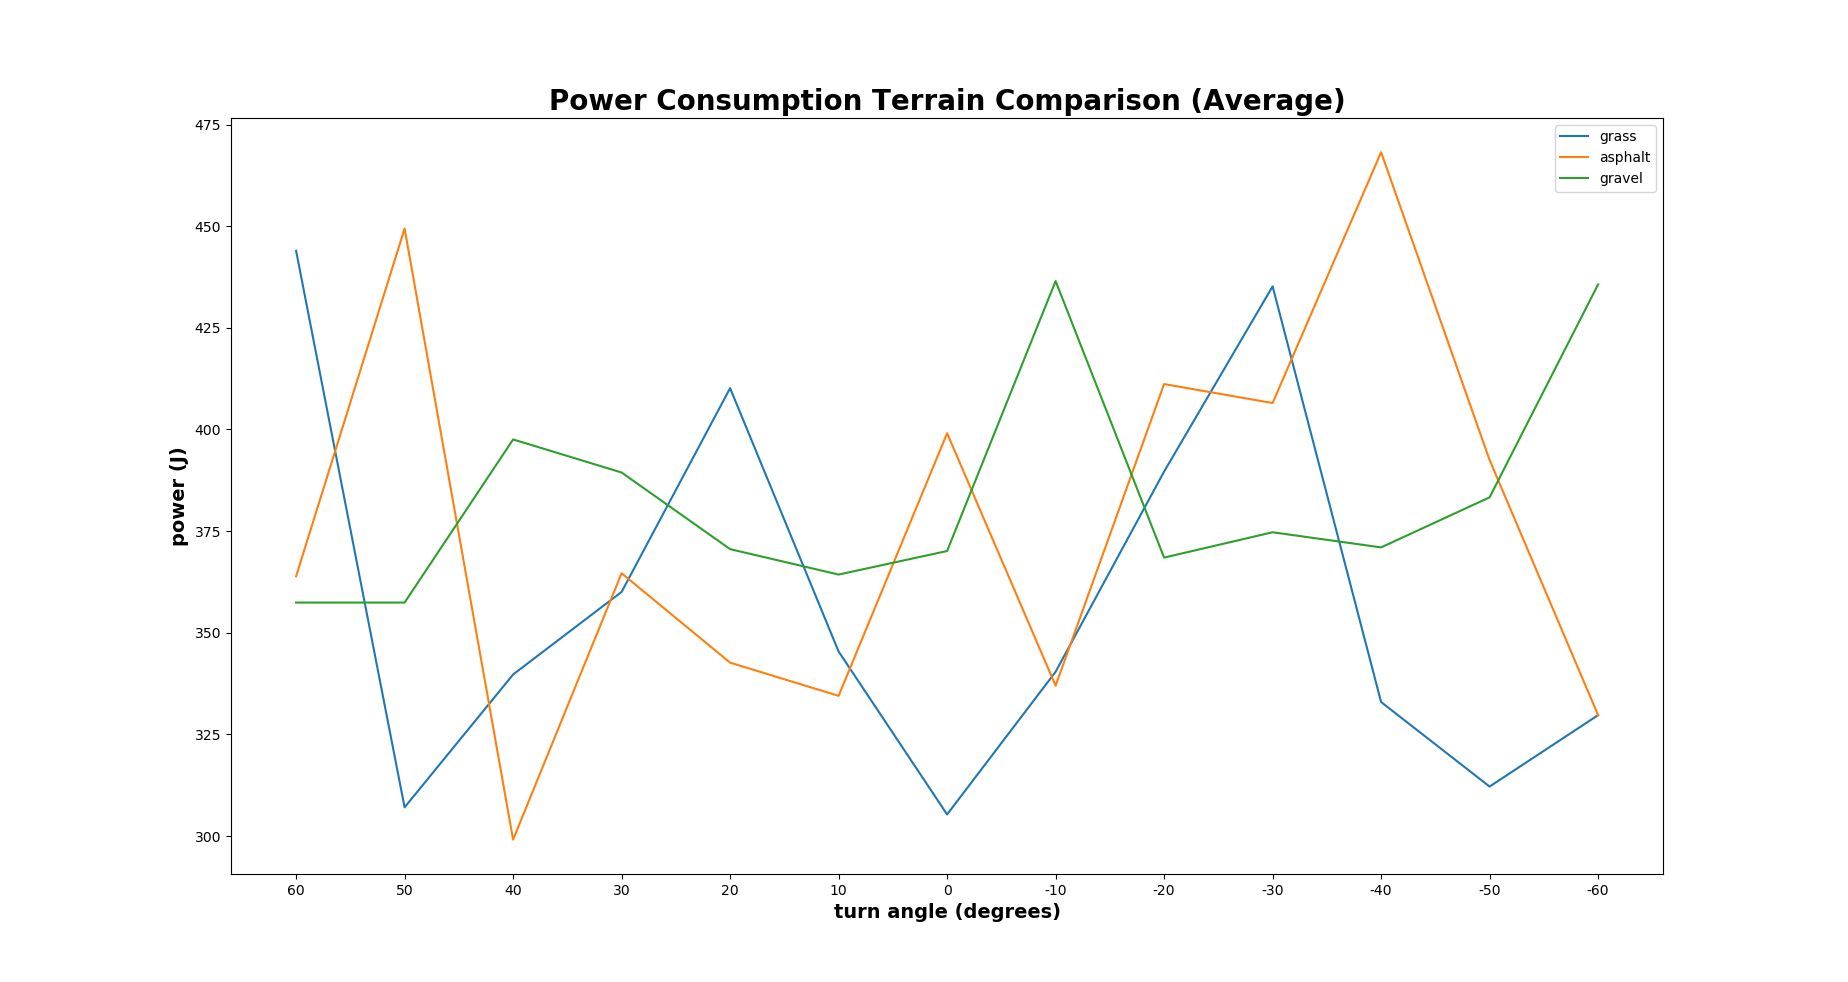
\includegraphics[width=1\linewidth]{power_terrains.png}
    \end{adjustbox}
    
    \subsection{Velocity}
    \begin{adjustbox}{center, caption={Velocity profile for a 60 degree (left) turn}, nofloat=figure}
            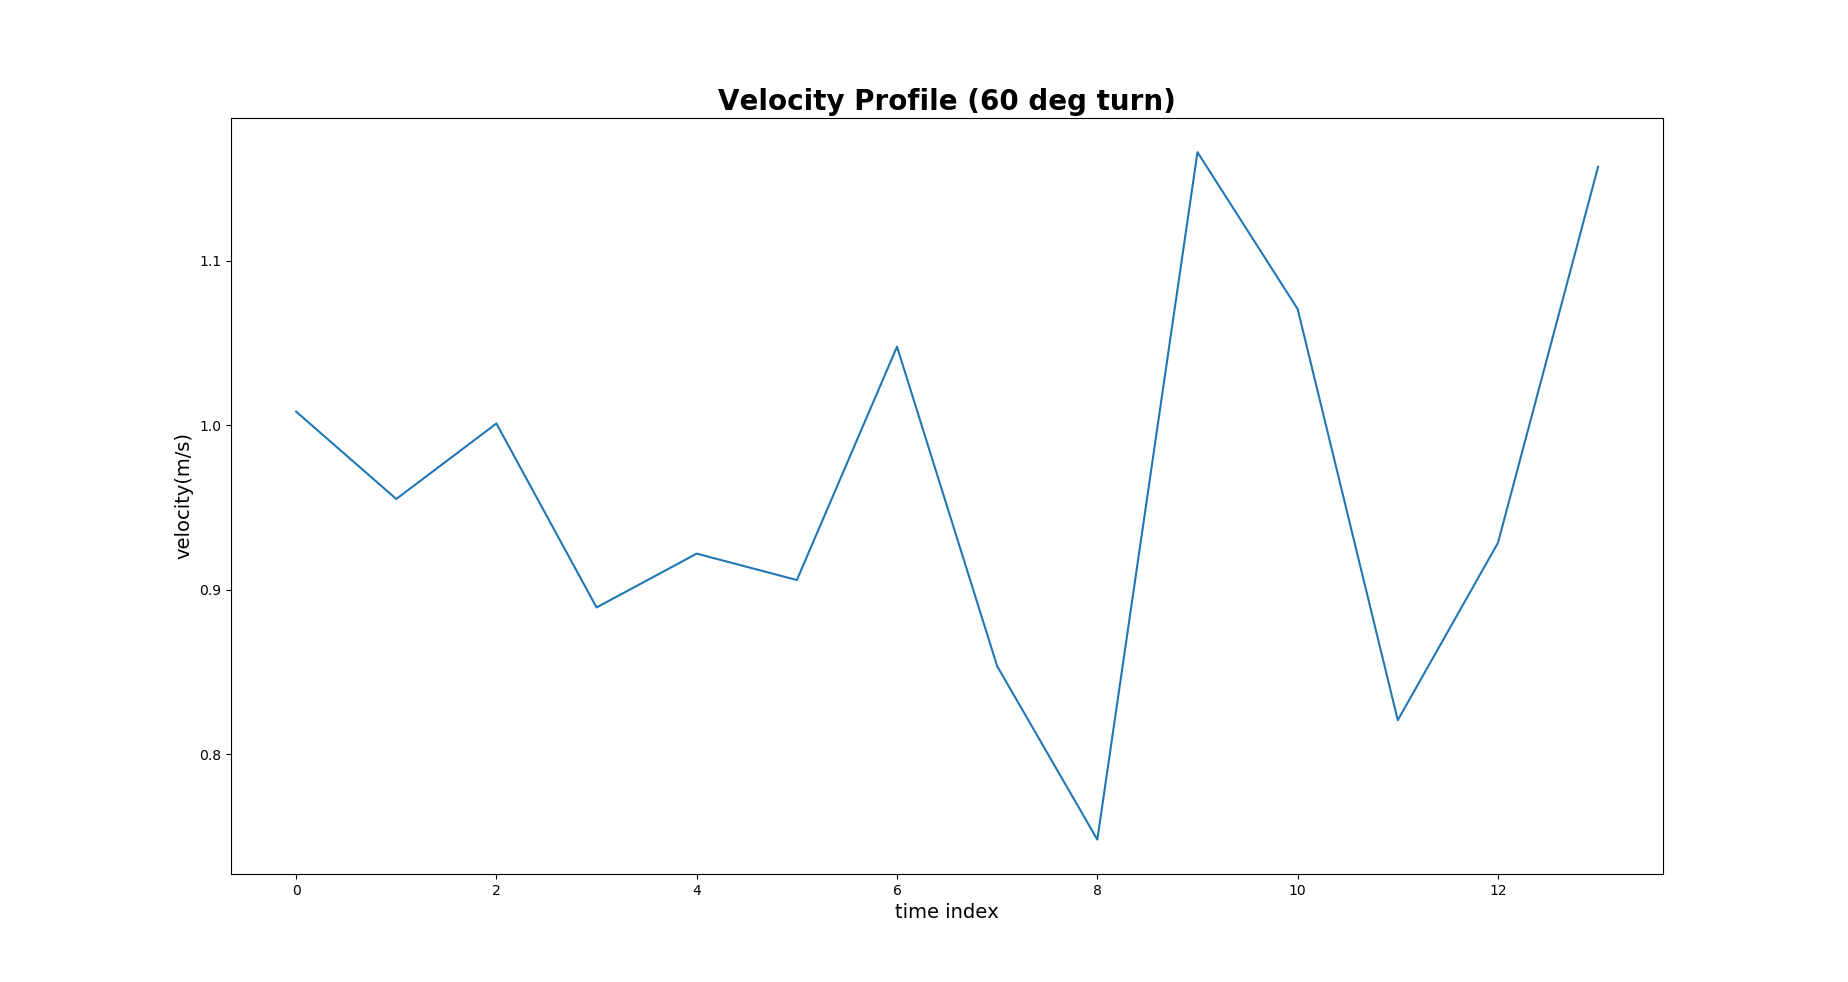
\includegraphics[width=1\linewidth]{velocity.png}
        \end{adjustbox}
    One potential theory for reduced power consumption at larger angles could be the robot slows down. Figure 8 shows velocity throughout the 5 seconds of turning left 60 degrees. The speed of the robot varies throughout the turn; however, it centers around the expected 1 m/s. Clearly more analysis and experiments are required to understand the profile. Perhaps robot characteristics lead to benefits at various turn angles.
    \noindent
        

\section{Conclusion}

    % results for terrain comparison show that energy costs vary 
    Our research has shown that energy consumption varies based on the terrain and angle that a robot is turning. These variables dramatically influence an energy efficient path planner like SBMPO but do not affect other path planners like A-Star. Due to these differences, we saw that SBMPO was able to create a more energy efficient path for SPOT. The only times that A-star and Dijkstra's were able to have similar scores to SBMPO was when the energy efficient route was the same as the shortest distance path. 
    
   Our research also found that SPOT does not have the usual power expenditure curve that most robots have. Spot had specific angles on different terrains that it consumed less energy than was expected. SBMPO is able to use these power consumption anomalies to create unique paths that most path planners would not implement. 
 
    % SBMPO is 
\section{Future Research}

    With SBMPO showing that it is able to accurately predict energy efficient paths, the next step forward is to have SBMPO detect the type of terrain underneath it and use that information to update its plan while moving. Current research into detecting the type of terrain that is beneath a legged robot using only motor information and a trained LSTM model looks like a promising way to help SPOT detect the terrain it is on \cite{christopher}. 
    
    Another area of focus is to speed up SBMPO's convergence speed so that it can be used in real time planning scenarios. Previous research has been done with speeding up SBMPO's path predicting time using a machine learned heuristic \cite{carter}.
    
    By implementing these two research goals we hope to create a usable real-time energy efficient path planner for legged robots.

\bibliographystyle{IEEEtranN}
\bibliography{refs}
\end{document}